\documentclass[a4paper,10pt,twocolumn]{article}

% =======================
% Packages
% =======================
\usepackage{amsmath, amssymb, amsthm, physics}
\usepackage{graphicx}
\usepackage{caption}
\captionsetup{font=small}
\usepackage{subcaption}
\usepackage{hyperref}
\usepackage{geometry}
\usepackage{float}
\usepackage{gensymb}
\usepackage{booktabs}
\usepackage{fancyhdr} % For custom headers/footers
\usepackage{indentfirst}
\usepackage[numbers]{natbib}  % if you want to control options explicitly
\setcitestyle{numbers,square}

\geometry{left=1.5cm, right=1.5cm, top=1.785cm, bottom=2.0cm}
\setlength{\parindent}{0in}
\sloppy

% =======================
% Header / Footer
% =======================
\pagestyle{fancy}
\fancyhf{}                     
\lhead{Computational Lab Report}
\rhead{Angze Li (CID: 02372394)}
\cfoot{\thepage}

\makeatletter
\let\ps@plain\ps@fancy        
\makeatother
% =======================
% Title
% =======================
\title{\textbf{Computational Lab Report: \\
Liquid Simulation}}
\author{Angze Li, CID: 02373494 \\
    Department of Chemistry, Imperial College London}

\begin{document}

\maketitle

% Abstract
\noindent
\twocolumn[
\begin{@twocolumnfalse}
\maketitle
\begin{abstract}
Abstract Abstract Abstract
\end{abstract}
\end{@twocolumnfalse}
]

\vspace{1em}

% =========================================================
\section{Introduction}  % ~20\% of total marks, limit to ~1.5 page

Introduction Introduction Introduction

\textit{Questions:}

\textit{1. Give a brief account on what molecular dynamics is, and (broadly speaking) what it aims to achieve. [5]}

\textit{2. Give two examples of instances where molecular dynamics simulations have/can be used (in a helpful way) instead of or in synergy with experimental techniques. In each case explain why. [10] (Please consider only chemically relevant examples. E.g. To study
geochemical processes which occur under extreme temperature/pressure conditions, and therefore difficult to study experimentally.)}

\textit{3. Computer simulations are performed under specific "experimental" conditions. The thermodynamic ensemble defines these conditions. Explain what is meant by the thermodynamic ensemble. Your answer should also provide three ensemble examples and briefly discuss what quantities are conserved in each ensemble. You may want to consult
Atkins' Physical Chemistry 11th edition (Focus 13D) to address this question. [5]}

% =========================================================
% 2. Exercises / Results & Discussion (~60%)
% =========================================================
\section{Results and Discussion} % ~60\%

\subsection{Introduction to molecular dynamics simulation}
\subsubsection*{TASK 1: By taking Taylor expansions of $x(t+\delta t)$ and $x(t-\delta t)$, write general expressions for them up to the fourth order $\mathcal{O}(t^4)$. Having written these expressions, derive the formula in Figure 2 used to update positions in the classical Verlet algorithm: $x_i(t+\delta t)\approx2x_i(t)-x_i(t-\delta t)+\frac{F_i(t)}{m}\,\delta t^2$ by using Newton’s second law to replace $\frac{d^2 x_i(t)}{dt^2}$. [4 marks]}

For a function $f(x)$ that is infinitely differentiable at $a$, Taylor expansion is defined as:
\[
f(a+\delta x)=\sum_{n=0}^{+\infty}\frac{f^{(n)}(a)}{n!}(\delta x)^n.
\]
Let $x_i(t+\delta t)$ denote the position of an arbitrary atom $i$ at time $t+\delta t$. Expanding $x_i(t+\delta t)$ up to the fourth order gives:
\[
x(t+\delta t)=x(t)+x'(t)\delta t+\frac{x''(t)}{2}(\delta t)^2+\frac{x'''(t)}{6}(\delta t)^3+\mathcal{O}(t^4).
\]
Since $x'(t)=v(t)$ and $x''(t)=a(t)$,
\[
x(t+\delta t)=x(t)+v(t)\delta t+\frac{a(t)}{2}(\delta t)^2+\frac{a'(t)}{6}(\delta t)^3+\mathcal{O}(t^4).
\]
Substituting $\delta t$ by $-\delta t$, we obtain
\[
x(t-\delta t)=x(t)-v(t)\delta t+\frac{a(t)}{2}(\delta t)^2-\frac{a'(t)}{6}(\delta t)^3+\mathcal{O}(t^4).
\]
Adding $x(t-\delta t)$ to $x(t+\delta t)$ gives
\[
x(t+\delta t)+x(t-\delta t)=2x(t)+a(t)(\delta t)^2+\mathcal{O}(t^4).
\]
Using Newton's law ($F(t)=ma(t)$) and omitting $\mathcal{O}(t^4)$, the equation becomes
\[
x(t+\delta t)+x(t-\delta t)\approx2x(t)+\frac{F(t)}{m}(\delta t)^2.
\]
By rearranging, we arrive at
\[
x(t+\delta t)\approx 2x(t)-x(t-\delta t)+\frac{F(t)}{m}(\delta t)^2,
\]
which is the formula used in the classic Verlet algorithm (CVA,~\cite{verlet1967computer}).

\subsubsection*{TASK 2: What could be an advantage of the Velocity-Verlet algorithm over the classical Verlet algorithm? [2 marks]}

The Velocity-Verlet algorithm (VVA,~\cite{swope1982computer}) lets us calculate the atom velocities explicitly by using
\[
v_i(t+\delta t)=v_i(t+\frac{1}{2}\delta t)+\frac{1}{2}a_i(t+\delta t)\delta t.
\]
Though when VVA is adopted, we need to specify the initial velocities apart from the initial positions, this algorithm comes with several advantages compared to the CVA. A number of physical, especially dynamical quantities depend on velocity, e.g., kinetic energy, temperature, where VVA allows accurate calculation of these quantities at each timestep without approximation. Additionally, while retaining the same global error, stochastic collisions of atoms can easily be implemented for the VVA algorithm as velocities are computed for the entire trajectory.~\cite{andersen1983rattle}

\subsubsection*{TASK 3: Consider the Lennard-Jones pair potential. What physical interaction(s) does it describe? What is the physical significance for the $r^{-6}$ and $r^{-12}$ terms? [3 marks]}
\begin{figure}
    \centering
    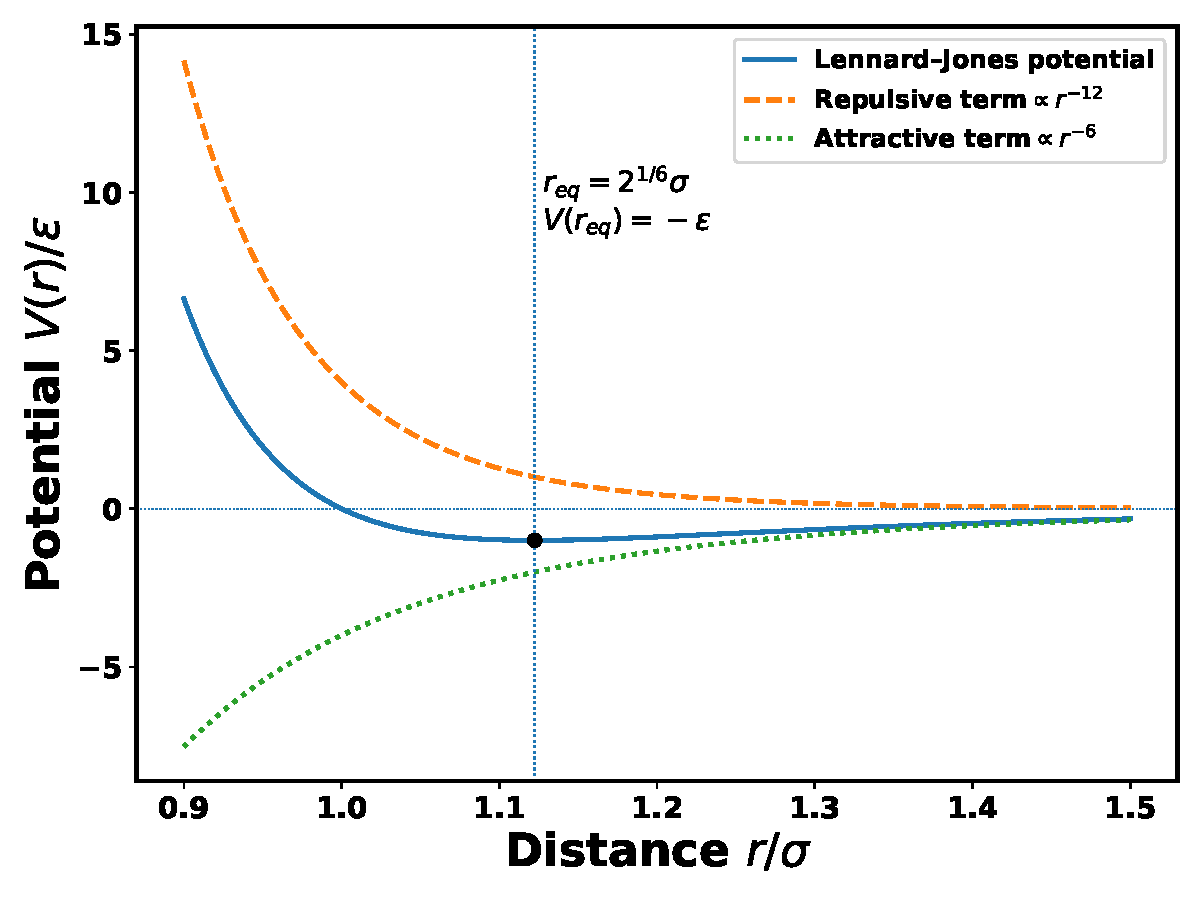
\includegraphics[width=1\linewidth]{Figures/lj_potential.pdf}
    \caption{Lennard–Jones potential showing the short-range repulsive $r^{-12}$ term and long-range attractive $r^{-6}$ dispersion interaction. The potential minimum occurs at $r_{eq}=2^{1/6}\sigma$, where the energy is $V(r_{eq})=-\varepsilon$. The well depth $\varepsilon$ represents the interaction strength between two particles.}
    \label{fig:lj_potential}
\end{figure}
The Lennard--Jones (LJ) pair potential describes the interaction between two neutral atoms or molecules through a combination of attractive and repulsive forces. It was first proposed in 1924 to describe the cohesive energy of crystals of noble gases,~\cite{jones1924determination} and has since been widely used to model intermolecular interactions in simple liquids and gases.~\cite{wang2020lennard}

The attractive $r^{-6}$ term represents long-range London dispersion (van der Waals) interactions arising from instantaneous dipole–induced dipole correlations between particles. The repulsive $r^{-12}$ term models the strong short-range repulsion that occurs when electron clouds overlap, which is primarily a consequence of the Pauli exclusion principle. The behaviours of the potential from the two terms at different distances are shown in Fig.~\ref{fig:lj_potential}.

The depth of the potential well, $\varepsilon$, represents the strength of the interaction between two particles and corresponds to the minimum potential energy at the equilibrium separation. Physically, it reflects the cohesive energy scale of the interaction and determines how strongly particles are bound in the system.

\subsubsection*{TASK 4: For a single Lennard--Jones interaction, $\phi(r)=4\varepsilon\left[\left(\frac{\sigma}{r}\right)^{12}-\left(\frac{\sigma}{r}\right)^6\right]$, find the separation $r_0$ at which the potential energy is zero. What is the force at this separation? Find the equilibrium separation $r_{\mathrm{eq}}$ and determine the well depth $\phi(r_{\mathrm{eq}})$. Evaluate the integrals $\int_{2\sigma}^{\infty}\phi(r)\,dr$, $\int_{2.5\sigma}^{\infty}\phi(r)\,dr$, and $\int_{3\sigma}^{\infty}\phi(r)\,dr$ when $\sigma=\varepsilon=1.0$.
[4 marks]}

Let $\phi(r)=0$, dividing both sides by $4\varepsilon$ and moving repulsive term to the RHS, we obtain
\[
\sigma^{12}{r}^{-12}=\sigma^{6}{r}^{-6}.
\]
Simple algebra gives
\[
r^{-6}=\sigma^{-6}
\]
and therefore $r_0=\sigma$, given both $r$ and $\sigma$ are positive.

The force at $r_0$ can be evaluated by taking the derivative of the LJ potential at $r_0$:
\begin{align*}
\frac{d\phi(r)}{d r}
&= 4\varepsilon\left(\sigma^{12}\cdot -12r^{-13}-\sigma^{6}\cdot -6r^{-7} \right)
\\
&= 4\varepsilon\left(-12\sigma^{12}r^{-13}+6\sigma^{6}r^{-7} \right).
\end{align*}
At $r=r_0$,
\begin{align*}
\frac{d\phi(r)}{d r}\Big|_{r=\sigma}
&= 4\varepsilon\left(-12\sigma^{-1}+6\sigma^{-1} \right)
\\
&= -24\varepsilon\sigma^{-1}.
\end{align*}
Therefore, the force at $r_0$ is 
\[
F(r_0)=-\frac{d\phi(r)}{d r}\Big|_{r=\sigma}=24\varepsilon\sigma^{-1},
\]
indicating a repulsive force at $r_0=\sigma$.

At the equilibrium separation ($r_{\mathrm{eq}}$), the derivative of the LJ potential, i.e., the force is 0. To find $r_{\mathrm{eq}}$, we can solve the equation 
\[
F=-4\varepsilon\left(-12\sigma^{12}r_{\mathrm{eq}}^{-13}+6\sigma^{6}r_{\mathrm{eq}}^{-7} \right)=0.
\]
Dividing both sides by $4\varepsilon$ and rearranging the equation gives
\[
6\sigma^{6}r_{\mathrm{eq}}^{-7}=12\sigma^{12}r_{\mathrm{eq}}^{-13}.
\]
With simple algebra, we can find that
\[
r_{\mathrm{eq}}=(2)^{1/6}\sigma,
\]
Substituting $r=r_{\mathrm{\mathrm{eq}}}$ into the LJ potential gives
\begin{align*}
\phi(r_{\mathrm{eq}})
&= 4\varepsilon\left[\left(\frac{\sigma}{r_{\mathrm{eq}}}\right)^{12}-\left(\frac{\sigma}{r_{\mathrm{eq}}}\right)^6\right]
\\
&= 4\varepsilon\left[\left(\frac{\sigma}{(2)^{1/6}\sigma}\right)^{12}-\left(\frac{\sigma}{(2)^{1/6}\sigma}\right)^6\right]
\\
&= 4\varepsilon\Big(\big(2^{-1/6}\big)^{12}-\big(2^{-1/6}\big)^{6}\Big)
\\
&= 4\varepsilon\cdot-2^{-2}
\\
&= -\varepsilon.
\end{align*}
Let $\sigma=\varepsilon=1.0$, the LJ potential becomes
\[
\phi(r)=4r^{-12}-4r^{-6}.
\]
The integral of this LJ potential with infinity as upper limit and $a$ (where $a>0$) as lower limit is
\begin{align*}
\int^{+\infty}_{a} \phi(r)\ dr
&= \Big[-\frac{4}{11}r^{-11}+\frac{4}{5}r^{-5}\Big]^{+\infty}_{a}
\\
&= 0-\Big[-\frac{4}{11}a^{-11}+\frac{4}{5}a^{-5}\Big]
\\
&= \frac{4}{11}a^{-11}-\frac{4}{5}a^{-5}.
\end{align*}
The integrals can then be evaluated as below:
\begin{align*}
\int_{2\sigma}^{\infty}\phi(r)\,dr
&= \frac{4}{11}\cdot2^{-11}-\frac{4}{5}\cdot2^{-5}
\approx -0.0248 \; (\text{to 3 s.f.}) \\
\int_{2.5\sigma}^{\infty}\phi(r)\,dr
&= \frac{4}{11}\cdot2.5^{-11}-\frac{4}{5}\cdot2.5^{-5}
\approx -0.00818 \; (\text{to 3 s.f.}) \\
\int_{3\sigma}^{\infty}\phi(r)\,dr
&= \frac{4}{11}\cdot3^{-11}-\frac{4}{5}\cdot3^{-5}
\approx -0.00329 \; (\text{to 3 s.f.})
\end{align*}
From these results, the magnitude of $\int_{a}^{\infty}\phi(r)\,dr$ decreases as the lower limit $a$ increases. This shows that the long-range contribution of the LJ potential becomes progressively smaller at larger separations, consistent with the fact that $\phi(r)\to 0$ as $r\to+\infty$.

\subsubsection*{TASK 5: Consider an atom at position $(0.5,\,0.5,\,0.5)$ in a cubic simulation box that spans from $(0,\,0,\,0)$ to $(1,\,1,\,1)$. In a single timestep, it moves along the vector $(0.7,\,0.6,\,0.2)$. At what position does the atom end up after applying periodic boundary conditions? [1 mark]}
After the atom moves, its position becomes
\[
(0.5,\,0.5,\,0.5)+ (0.7,\,0.6,\,0.2)=(1.2,\ 1.1,\ 0.7).
\] 
As the atom crosses the boundary of the simulation box, periodic boundary conditions map its position back into the box by subtracting the box length in the corresponding directions, and therefore, the atom ends up at
\[
(0.2,\ 0.1,\ 0.7).
\]
\subsubsection*{TASK 6: The Lennard--Jones parameters for argon are $\sigma = 0.34\,\mathrm{nm}$ and $\varepsilon/k_B = 120\,\mathrm{K}$. If the reduced LJ cutoff is $r^* = 3.2$, what is it in real units? What is the well depth in $\mathrm{kJ\,mol^{-1}}$? What is the reduced temperature $T^* = 1.5$ in real units? [1 mark]}
The LJ cutoff in meter is 
\[
r=r^*\sigma=3.2\cdot 0.34\ \mathrm{nm}=1.088\ \mathrm{nm}.
\]
The well depth in $\mathrm{J}$ is
\begin{align*}
\varepsilon(\mathrm{J}) &= k_B \cdot 120\,\mathrm{K} =1.381\times10^{-23}\,\mathrm{J\,K^{-1}}\cdot120\,\mathrm{K} 
\\
&=  1.6572\times10^{-21}\,\mathrm{J}.
\end{align*}
To obtain the well depth in $\mathrm{kJ\,mol^{-1}}$, we can multiply $\varepsilon$ by Avogadro's number and converting J to kJ:
\begin{align*}
\varepsilon(\mathrm{kJ\,mol^{-1}}) 
&= \varepsilon(\mathrm{J})\cdot10^{-3}\ \mathrm{kJ\ J^{-1}}\cdot N_A
\\
&=  1.6572\times10^{-24}\,\mathrm{kJ}\cdot 6.022\times10^{23}\ \mathrm{mol^{-1}}
\\
&\approx 0.997\ \mathrm{kJ\ mol^{-1}}\ (\text{to 3 s.f.}).
\end{align*}
\subsection{Equilibration}
\subsubsection*{What does it mean for a simulation to ``reach equilibrium''? Why is this important in terms of sampling from an ensemble using molecular dynamics? [2]
Plot the energy (potential, kinetic and total), temperature and pressure, against time for the 0.001 timestep experiment [2] }

The simulated system reaches equilibrium when its macroscopic quantities (i.e., temperature, pressure and energy) fluctuate around the stable average values. At this stage, the system has reached a steady thermodynamic state consistent with the specified ensemble.

This is important because MD samples configurations in a statistical way in the ensemble only after the system has equilibrated. If the simulation has not reached equilibrium, the sampled configurations may still reflect the initial conditions rather than the true equilibrium distribution, leading to incorrect averages of physical properties.


\subsubsection*{Does the simulation reach equilibrium? How can you tell? [2] }
The simulation has reached equilibrium. From Fig.~\ref{fig:equilibration}, the thermodynamic quantities fluctuate around approximately constant mean values without systematic drift. In particular, the temperature and pressure fluctuate around the target reduced values ($T^* = 1.5$, $P^* = 1$) specified in the input file. The potential, kinetic, and total energies also exhibit stationary fluctuations after a short initial relaxation period. These observations indicate that the system has equilibrated.

\subsubsection*{
Plot the energy (potential, kinetic and total), temperature and pressure, against time for the 0.001 timestep experiment [2] }
\begin{figure}[H]
\centering

\begin{subfigure}{0.9\linewidth}
\centering
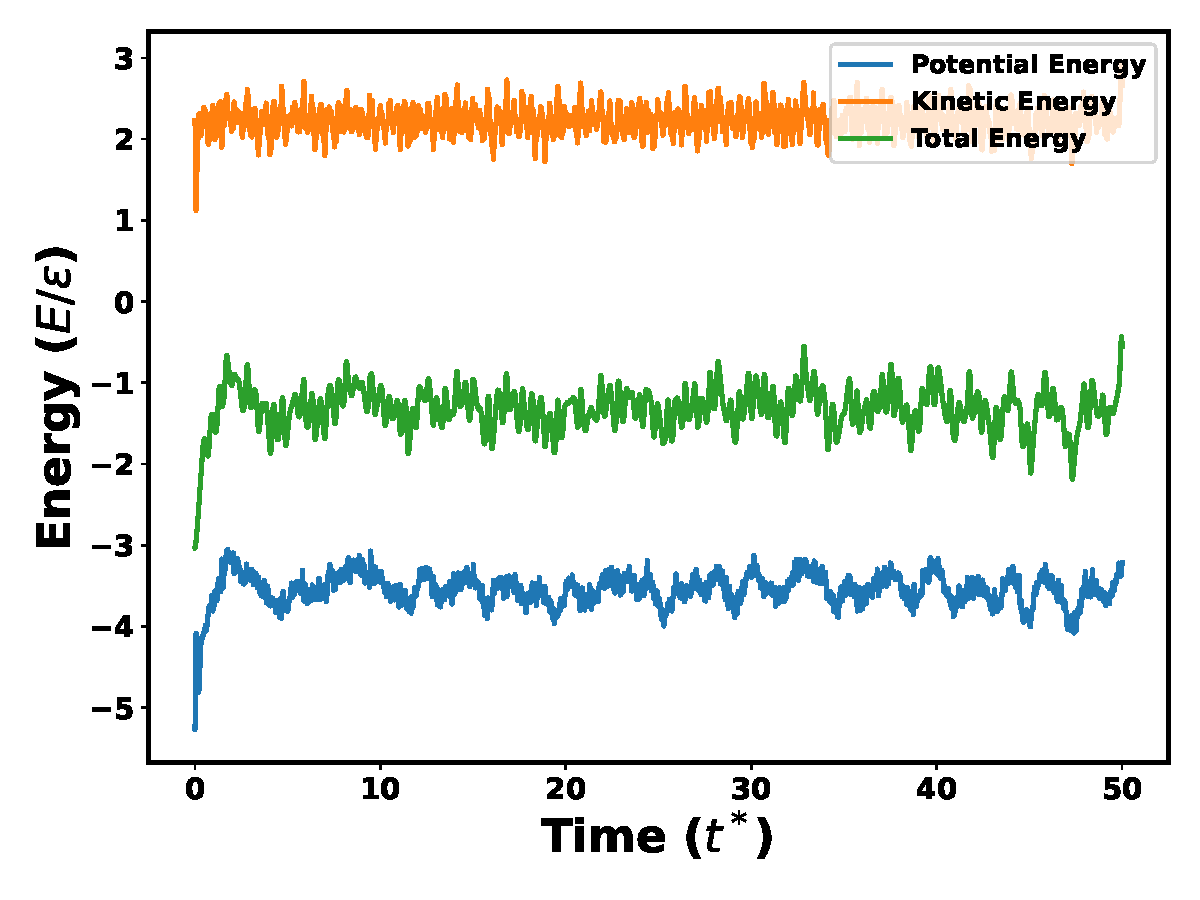
\includegraphics[width=\linewidth]{Figures/energy_vs_time_ts0.001.pdf}
\caption{Potential, kinetic, and total energy vs time.}
\end{subfigure}
\vspace{0.2cm}

\begin{subfigure}{0.9\linewidth}
\centering
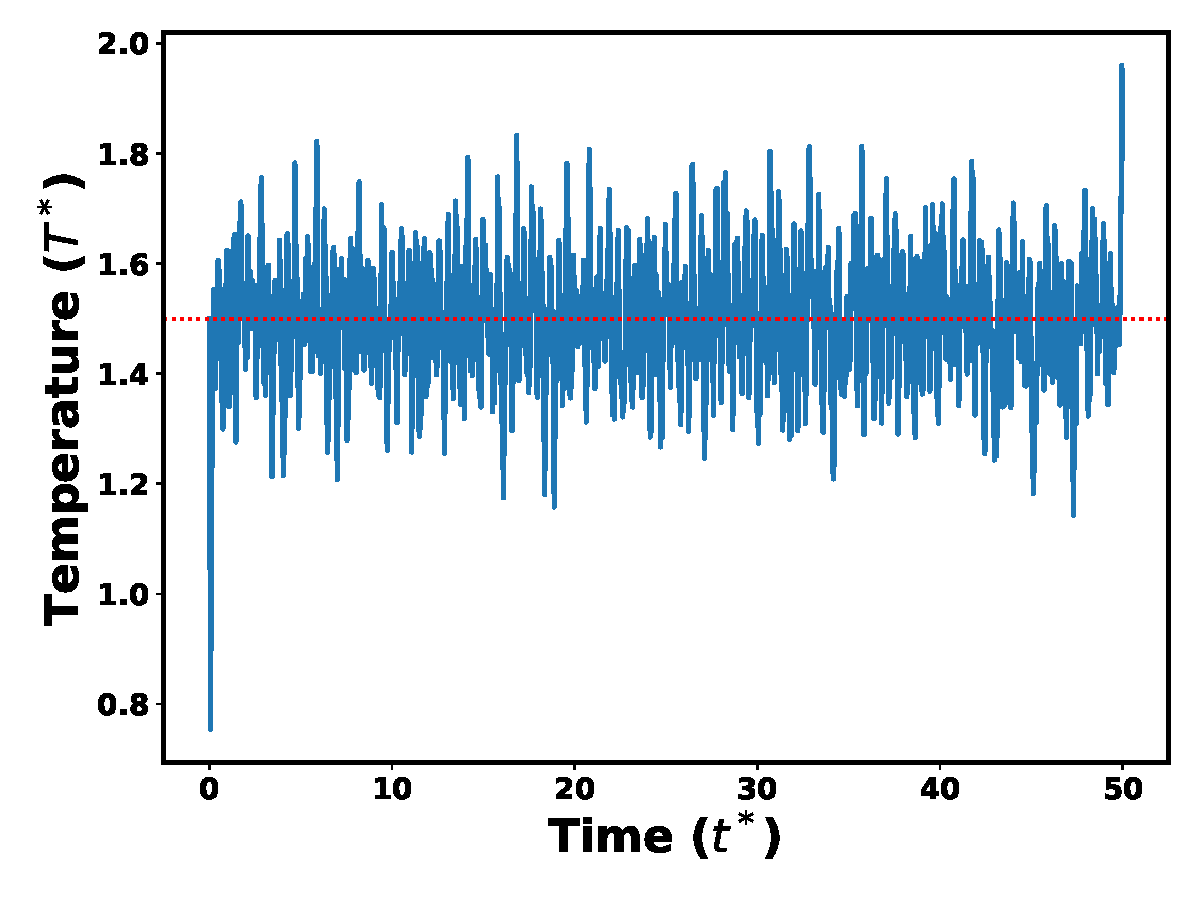
\includegraphics[width=\linewidth]{Figures/temperature_vs_time_ts0.001.pdf}
\caption{Temperature vs time ($T^*=1.5$).}
\end{subfigure}
\vspace{0.2cm}

\begin{subfigure}{0.9\linewidth}
\centering
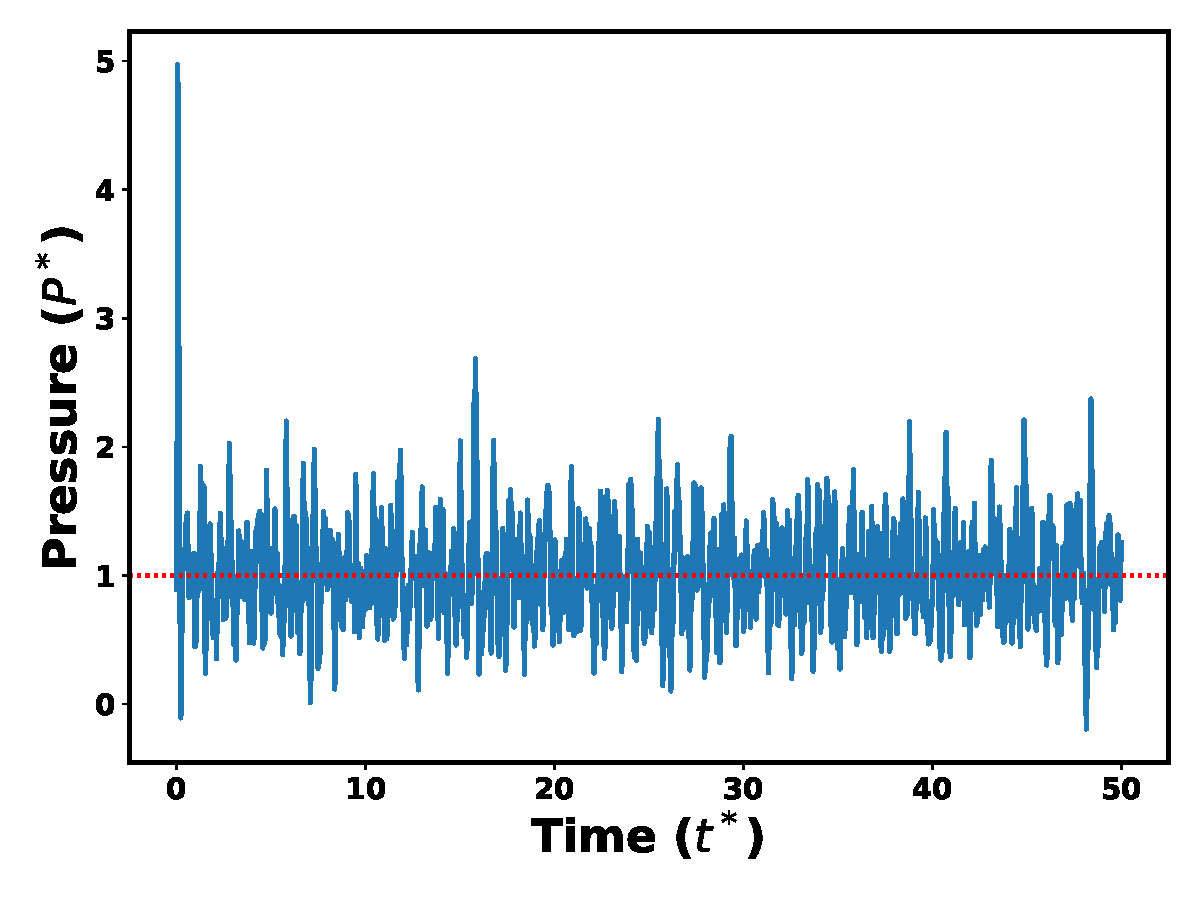
\includegraphics[width=\linewidth]{Figures/pressure_vs_time_ts0.001.pdf}
\caption{Pressure vs time ($P^*=1$).}
\end{subfigure}

\caption{Thermodynamic properties of the system during the NPT simulation with timestep $0.001$.}
\label{fig:equilibration}
\end{figure}


\subsubsection*{Make a single plot which shows the energy vs. time for the timesteps you have simulated [2].}
\begin{figure}[H]
    \centering
    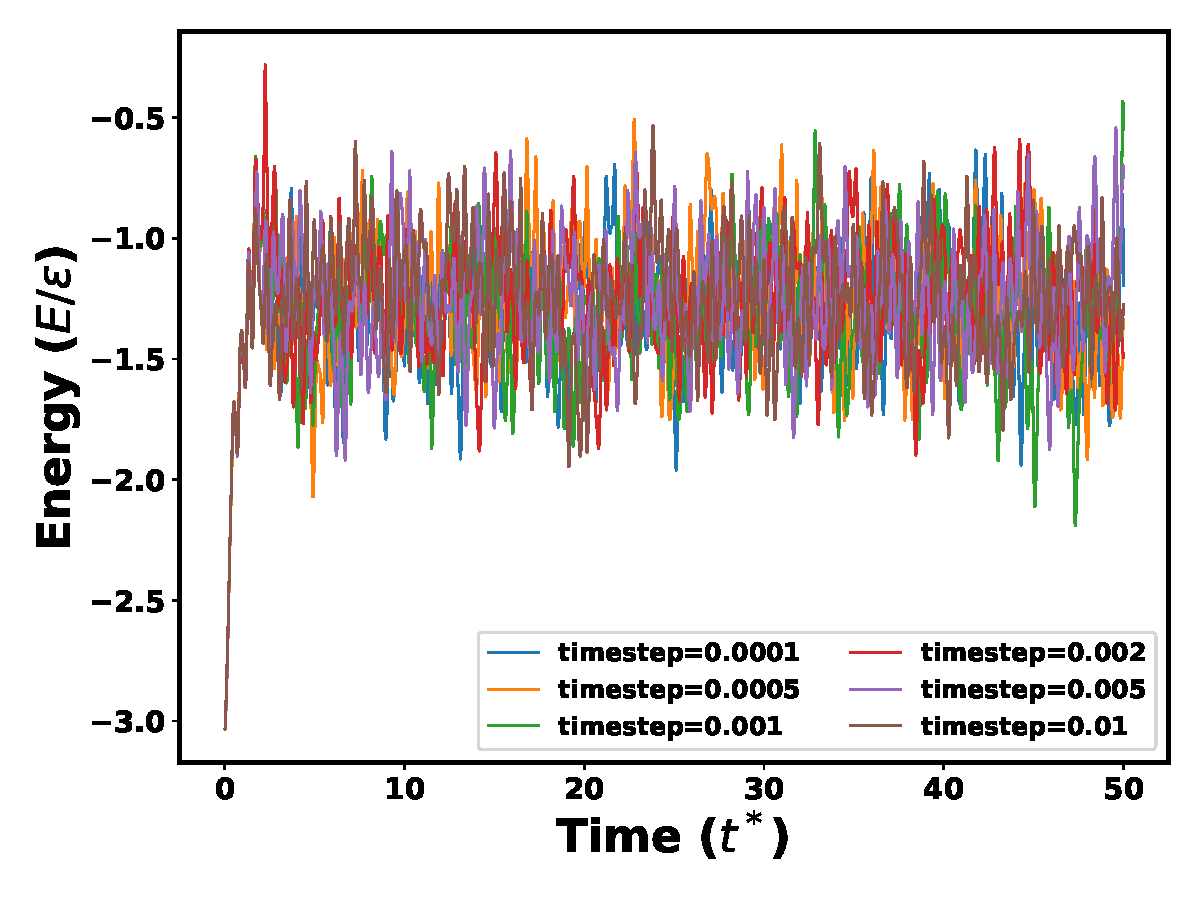
\includegraphics[width=0.9\linewidth]{Figures/energy_vs_time_different_ts.pdf}
    \caption{Total energy as a function of simulation time for NPT simulations with different timesteps. After equilibration, the energy fluctuates around a stable mean value for all tested timesteps, indicating numerical stability.}
    \label{fig:energy_vs_time_different_ts}
\end{figure}

\subsubsection*{Of the timesteps that you used, which timestep will you use for subsequent simulations and why? [6]}
\begin{figure}[H]
    \centering
    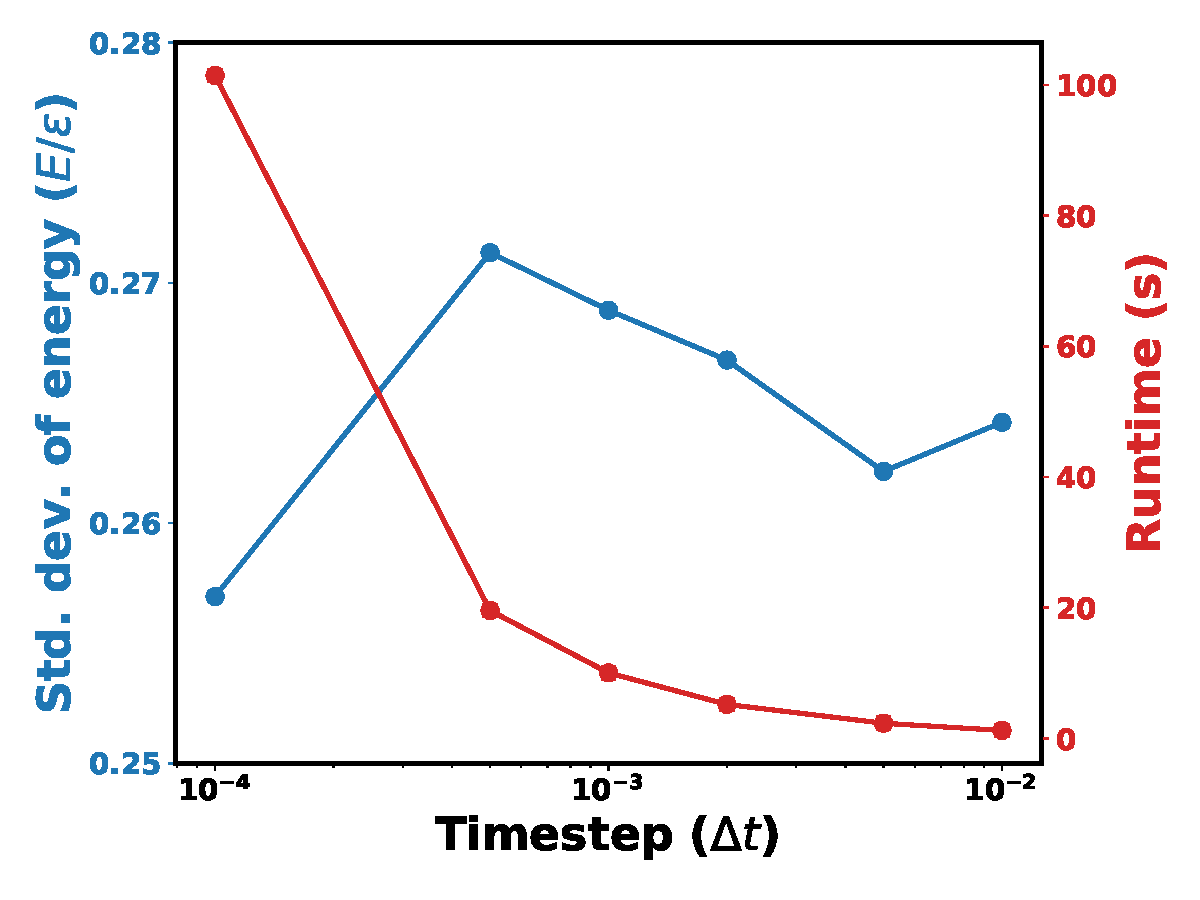
\includegraphics[width=0.9\linewidth]{Figures/timestep_stability_runtime.pdf}
    \caption{Standard deviation of the total energy (blue, left axis) and simulation runtime (red, right axis) as a function of integration timestep. The energy fluctuations remain similar across the tested timesteps, indicating numerical stability, while the computational runtime decreases rapidly with increasing timestep.}
    \label{fig:energy_vs_time_different_ts}
\end{figure}

\subsection{Running simulations under specific conditions}

\subsection{Structural properties and the radial distribution function}

\subsection{Dynamical properties and the diffusion coefficient}
% =========================================================
% 3. Conclusions (~20%)
% =========================================================
\section{Conclusions} % ~20\% of total marks, limit to ~1.5 page
Conclusions Conclusions Conclusions

\textit{Questions}

\textit{1. In this lab, you have used the Lennard-Jones potential exclusively. Give one example of a system that can be described well using only LJ potentials. What additional elements would you need to add to the interaction potential to model a molecule, e.g. water? [6]}

\textit{2. What cut-off have you been using in your simulations? What are the advantages and disadvantages for using a shorter/longer cut-off? (Hint: consider here the balance of computational cost vs accuracy in describing the properties of a system.) [3]}

\textit{3. In this lab you have investigated the properties of solids, liquids and gases. Would you observe a liquid phase (and by extension a critical point) if the LJ interaction strength, $\varepsilon$, is
very weak? What interaction strength is required to generate a liquid phase? (Hint: to address this question you may want to revise the 2nd year Solids, Liquid and Interfaces lecture notes - see "Phase transitions of pure substances") [4]}

\textit{4. What are finite size effects? Do you think they are significant in the simulations you have performed? Why? [3]}

\textit{5. Algorithms such as SHAKE and RATTLE are widely used to model molecular systems as they allow MD simulations to be performed while fixing bond lengths. Why is this desirable? [4] (Hint: think about the timestep.)}

    
% =========================================================
% References
% =========================================================
%\section*{References}
{\small
\setlength{\bibsep}{0pt}
\bibliographystyle{achemso}
\bibliography{references}
}

\onecolumn 

\newpage
\section*{Supporting Information} 
\setcounter{figure}{0}
\renewcommand{\thefigure}{S\arabic{figure}}
\setcounter{table}{0}
\renewcommand{\thetable}{S\arabic{table}}
\setcounter{page}{1}
\renewcommand{\thepage}{S\arabic{page}}

Supporting Information Supporting Information Supporting Information

\end{document}